\section{Representation}

\subsection{Nodes}
Nodes for the main decision tree, or ADFs, comprise decision and end nodes. Decision nodes take a number of children and select one of them based on the value of a patient's attribute. There are 7 decision nodes - one for each attribute, excluding \emph{COMFORT} as it contains missing values. The number of children for decision nodes depends on the possible values for their associated attributes. The Blood Pressure (\emph{BP}) node, for instance, has 3 children - one for \emph{low}, one for \emph{mid} and one for \emph{high}. End nodes represent one of the three discharge decisions (\emph{I}, \emph{S} or \emph{A}); or, in the main decision-tree, end nodes may also reference one of 3 ADFs. The representation of ADFs is further explained in section \ref{sec:individuals}. The end nodes and decision nodes are described in table \ref{tab:nodes}.

\begin{table}[H]
\resizebox{\textwidth}{!}{\begin{tabular}{|l|l|l|}
\hline
\textbf{Symbol} & \textbf{Arity} & \textbf{Description}                                                                                                                                                                                                                                                                                                                                                                           \\ \hline
IT              & 3              & \begin{tabular}[c]{@{}l@{}}The internal temperature decision node\\ - If the patient's internal temperature is low then select the first child\\ - If the patient's internal temperature is mid then select the second child\\ - If the patient's internal temperature is high then select the third child\end{tabular}                                                                        \\ \hline
ITS             & 3              & \begin{tabular}[c]{@{}l@{}}The internal temperature stability decision node\\ - If the patient's internal temperature is unstable then select the first child\\ - If the patient's internal temperature is moderately stable then select the second child\\ If the patient's internal temperature is stable then select the third child\end{tabular}                                           \\ \hline
ST              & 3              & \begin{tabular}[c]{@{}l@{}}The surface temperature decision node\\ - If the patient's surface temperature is low then select the first child\\ - If the patient's surface temperature is mid then select the second child\\ - If the patient's surface temperature is high then select the third child\end{tabular}                                                                            \\ \hline
STS             & 3              & \begin{tabular}[c]{@{}l@{}}The surface temperature stability decision node\\ - If the patient's surface temperature is unstable then select the first child\\ - If the patient's surface temperature is moderately stable then select the second child\\ - If the patient's surface temperature is stable then select the third child\end{tabular}                                             \\ \hline
BP              & 3              & \begin{tabular}[c]{@{}l@{}}The blood pressure decision node\\ - If the patient's blood pressure is low then select the first child\\ - If the patient's blood pressure is mid then select the second child\\ - If the patient's blood pressure is high then select the third child\end{tabular}                                                                                                \\ \hline
BPS             & 3              & \begin{tabular}[c]{@{}l@{}}The blood pressure stability decision node\\ - If the patient's blood pressure is unstable then select the first child\\ - If the patient's blood pressure is moderately stable then select the second child\\ - If the patient's blood pressure is stable then select the third child\end{tabular}                                                                 \\ \hline
OS              & 4              & \begin{tabular}[c]{@{}l@{}}The oxygen saturation decision node\\ - If the patient's oxygen saturation is poor then select the first child\\ - If the patient's oxygen saturation is fair then select the second child\\ - If the patient's oxygen saturation is good then select the third child\\ - If the patient's oxygen saturation is excellent then select the fourth child\end{tabular} \\ \hline
I               & 0              & The end node for the patient to be sent to an intensive care unit                                                                                                                                                                                                                                                                                                                              \\ \hline
S               & 0              & The end node for the patient to be sent home                                                                                                                                                                                                                                                                                                                                                   \\ \hline
A               & 0              & The end node for the patient to be sent to the general hospital floor                                                                                                                                                                                                                                                                                                                          \\ \hline
ADF0            & 0              & Returns the result of executing the first ADF of the individual.                                                                                                                                                                                                                                                                                                                               \\ \hline
ADF1            & 0              & Returns the result of executing the second ADF of the individual.                                                                                                                                                                                                                                                                                                                              \\ \hline
ADF2            & 0              & Returns the result of executing the third ADF of the individual.                                                                                                                                                                                                                                                                                                                               \\ \hline
\end{tabular}}
\caption{Decision Tree Nodes}
\label{tab:nodes}
\end{table}

\subsection{Individuals}\label{sec:individuals}
Each chromosome within a population consists of a 4 decision trees for determining the discharge decision for a patient. As per the architecture implemented by Bruce \cite{bruce1995application}, the first decision tree represents the main program while the other three trees represent ADFs.

The function set and terminal set for the main program are made up of all the available nodes in table \ref{tab:nodes}. For the ADFs the terminal sets all consist of only \emph{I}, \emph{S} and \emph{A} - hence, there are no references between the function-defining trees. In addition - the function set for the first ADF consists of \emph{BP} and \emph{BPS}, the function set for the second ADF consists of \emph{IT} and \emph{ITS}, and the function set for the third ADF consists of \emph{ST} and \emph{STS}.

Given the function and terminal sets described above for the main program and each ADF, an example of an individual is depicted in figure \ref{fig:individual}.

\begin{figure}[H]
\centering
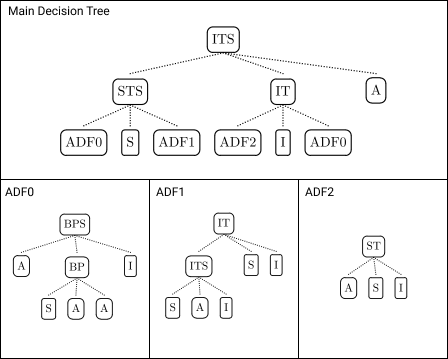
\includegraphics[width=\textwidth]{report/02_representation/chromosome.png}
\caption{Example of an Individual}
\label{fig:individual}
\end{figure}


\subsection{Populations}
Population representation and generation is the same as that applied by the previous genetic programming approach that did not incorporate modularization. To reiterate, the genetic algorithm made use of a single population consisting of 2048 individuals. This means that only a single population was evolved and cross-population breeding was not applied.

The initial population was generated using the ramped-half-and-half method proposed by Koza \cite{koza1992genetic} to enhance population diversity of structure. The maximum tree depth allowed during the initial population generation was 4. So, in other words, the population is divided equally among individuals to be initialized with trees having depths 2, 3, and 4. For each depth group, half of the trees are initialized with the full technique and half with the grow technique.

In addition, to cover as much of the search space as possible an effort was made to reduce duplicates within the initial population. The strategy used to reduce the number of duplicates was as follows: if a duplicate individual is created as part of the initial population, it will be regenerated up to 100 times to try replace it with a new, original individual. After 100 attempts, if no unique individual was generated, the duplicate individual will be used.